%File: anonymous-submission-latex-2023.tex
\documentclass[letterpaper]{article} % DO NOT CHANGE THIS
\usepackage{aaai23}  % DO NOT CHANGE THIS
\usepackage{times}  % DO NOT CHANGE THIS
\usepackage{helvet}  % DO NOT CHANGE THIS
\usepackage{courier}  % DO NOT CHANGE THIS
\usepackage[hyphens]{url}  % DO NOT CHANGE THIS
\usepackage{graphicx} % DO NOT CHANGE THIS
\usepackage{color}
\urlstyle{rm} % DO NOT CHANGE THIS
\def\UrlFont{\rm}  % DO NOT CHANGE THIS
\usepackage{natbib}  % DO NOT CHANGE THIS AND DO NOT ADD ANY OPTIONS TO IT
\usepackage{caption} % DO NOT CHANGE THIS AND DO NOT ADD ANY OPTIONS TO IT
\frenchspacing  % DO NOT CHANGE THIS
\setlength{\pdfpagewidth}{8.5in} % DO NOT CHANGE THIS
\setlength{\pdfpageheight}{11in} % DO NOT CHANGE THIS
%
% These are recommended to typeset algorithms but not required. See the subsubsection on algorithms. Remove them if you don't have algorithms in your paper.
%\usepackage{algorithm}
%\usepackage{algorithmic}
\newcommand{\sd}[1]{\textcolor{red}{[#1 \textsc{--Srijita}]}}

%
% These are are recommended to typeset listings but not required. See the subsubsection on listing. Remove this block if you don't have listings in your paper.
\usepackage{newfloat}
\usepackage{listings}
\DeclareCaptionStyle{ruled}{labelfont=normalfont,labelsep=colon,strut=off} % DO NOT CHANGE THIS
\lstset{%
	basicstyle={\footnotesize\ttfamily},% footnotesize acceptable for monospace
	numbers=left,numberstyle=\footnotesize,xleftmargin=2em,% show line numbers, remove this entire line if you don't want the numbers.
	aboveskip=0pt,belowskip=0pt,%
	showstringspaces=false,tabsize=2,breaklines=true}
%\floatstyle{ruled}
%\newfloat{listing}{tb}{lst}{}
%\floatname{listing}{Listing}
%
% Keep the \pdfinfo as shown here. There's no need
% for you to add the /Title and /Author tags.
\pdfinfo{
/TemplateVersion (2023.1)
}

\usepackage{xcolor}
\newcommand{\MET}[1]{\textcolor{blue}{MET: #1}}

 
% DISALLOWED PACKAGES
% \usepackage{authblk} -- This package is specifically forbidden
% \usepackage{balance} -- This package is specifically forbidden
% \usepackage{color (if used in text)
% \usepackage{CJK} -- This package is specifically forbidden
% \usepackage{float} -- This package is specifically forbidden
% \usepackage{flushend} -- This package is specifically forbidden
% \usepackage{fontenc} -- This package is specifically forbidden
% \usepackage{fullpage} -- This package is specifically forbidden
% \usepackage{geometry} -- This package is specifically forbidden
% \usepackage{grffile} -- This package is specifically forbidden
% \usepackage{hyperref} -- This package is specifically forbidden
% \usepackage{navigator} -- This package is specifically forbidden
% (or any other package that embeds links such as navigator or hyperref)
% \indentfirst} -- This package is specifically forbidden
% \layout} -- This package is specifically forbidden
% \multicol} -- This package is specifically forbidden
% \nameref} -- This package is specifically forbidden
% \usepackage{savetrees} -- This package is specifically forbidden
% \usepackage{setspace} -- This package is specifically forbidden
% \usepackage{stfloats} -- This package is specifically forbidden
% \usepackage{tabu} -- This package is specifically forbidden
% \usepackage{titlesec} -- This package is specifically forbidden
% \usepackage{tocbibind} -- This package is specifically forbidden
% \usepackage{ulem} -- This package is specifically forbidden
% \usepackage{wrapfig} -- This package is specifically forbidden
% DISALLOWED COMMANDS
% \nocopyright -- Your paper will not be published if you use this command
% \addtolength -- This command may not be used
% \balance -- This command may not be used
% \baselinestretch -- Your paper will not be published if you use this command
% \clearpage -- No page breaks of any kind may be used for the final version of your paper
% \columnsep -- This command may not be used
% \newpage -- No page breaks of any kind may be used for the final version of your paper
% \pagebreak -- No page breaks of any kind may be used for the final version of your paperr
% \pagestyle -- This command may not be used
% \tiny -- This is not an acceptable font size.
% \vspace{- -- No negative value may be used in proximity of a caption, figure, table, section, subsection, subsubsection, or reference
% \vskip{- -- No negative value may be used to alter spacing above or below a caption, figure, table, section, subsection, subsubsection, or reference

\setcounter{secnumdepth}{0} %May be changed to 1 or 2 if section numbers are desired.

% The file aaai23.sty is the style file for AAAI Press
% proceedings, working notes, and technical reports.
%

% Title

% Your title must be in mixed case, not sentence case.
% That means all verbs (including short verbs like be, is, using,and go),
% nouns, adverbs, adjectives should be capitalized, including both words in hyphenated terms, while
% articles, conjunctions, and prepositions are lower case unless they
% directly follow a colon or long dash
\title{Augmenting Flight Training with AI to Efficiently Train Pilots}
\author {
     % Authors
     Michael Guevarra\textsuperscript{\rm 1},
     Srijita Das\textsuperscript{\rm 2,3},
     Christabel Wayllace\textsuperscript{\rm 2,3},
     Carrie Demmans Epp\textsuperscript{\rm 2},\\
     Matthew E.~Taylor\textsuperscript{\rm 2,3},
     Alan Tay\textsuperscript{\rm 1}
 }
 \affiliations {
     % Affiliations
     \textsuperscript{\rm 1}  Delphi Technology Corp:  \texttt{guevarrm@myumanitoba.ca}, \texttt{alantay@delphitechcorp.com}\\
     \textsuperscript{\rm 2} University of Alberta: \{\texttt{srijita1, wayllace, demmanse, matthew.e.taylor}\}@\texttt{ualberta.ca}\\
     \textsuperscript{\rm 3} Alberta Machine Intelligence Institute (Amii)
}


%\author{
%    %Authors
%    % All authors must be in the same font size and format.
%    Written by AAAI Press Staff\textsuperscript{\rm 1}\thanks{With help from the AAAI Publications %Committee.}\\
%    AAAI Style Contributions by Pater Patel Schneider,
%    Sunil Issar,\\
%    J. Scott Penberthy,
%    George Ferguson,
%    Hans Guesgen,
%    Francisco Cruz\equalcontrib,
%    Marc Pujol-Gonzalez\equalcontrib
%}

%\affiliations{
%    %Afiliations
%    \textsuperscript{\rm 1}Association for the Advancement of Artificial Intelligence\\
    % If you have multiple authors and multiple affiliations
    % use superscripts in text and roman font to identify them.
    % For example,

    % Sunil Issar, \textsuperscript{\rm 2}
    % J. Scott Penberthy, \textsuperscript{\rm 3}
    % George Ferguson,\textsuperscript{\rm 4}
    % Hans Guesgen, \textsuperscript{\rm 5}.
    % Note that the comma should be placed BEFORE the superscript for optimum readability

%    1900 Embarcadero Road, Suite 101\\
%    Palo Alto, California 94303-3310 USA\\
    % email address must be in roman text type, not monospace or sans serif
%    publications23@aaai.org
%
% See more examples next
%}

%Example, Single Author, ->> remove \iffalse,\fi and place them surrounding AAAI title to use it
% \iffalse
% \title{My Publication Title --- Single Author}
% \author {
%     Author Name
% }
% \affiliations{
%     Affiliation\\
%     Affiliation Line 2\\
%     name@example.com
% }

% \fi

% \iffalse
%Example, Multiple Authors, ->> remove \iffalse,\fi and place them surrounding AAAI title to use it
% \title{My Publication Title --- Multiple Authors}
% \author {
%     % Authors
%     Michael Guevarra,\textsuperscript{\rm 1}
%     Srijita Das, \textsuperscript{\rm 2}
%     Christabel Wayllace, \textsuperscript{\rm 2}
%     Carrie Demmans Epp, \textsuperscript{\rm 2}
%     Matthew E Taylor, \textsuperscript{\rm 2}
%     Alan Tay, \textsuperscript{\rm 1}
% }
% \affiliations {
%     % Affiliations
%     \textsuperscript{\rm 1}  Delphi Technology Corp\\
%     \textsuperscript{\rm 2} University of Alberta\\
%     \textsuperscript{\rm 3} University of Manitoba\\
%     guevarrm@myumanitoba.ca, srijita1@ualberta.ca, wayllace@ualberta.ca,alantay@delphitechcorp.com,matthew.e.taylor@ualberta.ca
% }

% \fi

% REMOVE THIS: bibentry
% This is only needed to show inline citations in the guidelines document. You should not need it and can safely delete it.
%\usepackage{bibentry}
% END REMOVE bibentry

\begin{document}

\maketitle

\begin{abstract}
We propose an AI-based pilot trainer to help students learn how to fly aircraft. First, an AI agent uses behavioral cloning to learn flying maneuvers from qualified flight instructors. Later, the system uses the agent's decisions to detect errors made by students and provide feedback to help students correct their errors. This paper presents an instantiation of the pilot trainer. We focus on teaching straight and level flying maneuvers by automatically providing formative feedback to the human student. 
\end{abstract}

%\section{Introduction}

There is a critical shortage of commercial pilots worldwide: according to~\citet{Wyman:22}, there will be a global gap of 34,000 pilots by 2025. Part of the problem is that pilots qualified to conduct such training are in very high demand and in short supply. Currently, human instructors guide trainees using flight simulator exercises. We posit that training an AI-enabled system to provide instruction for some tasks is a viable approach to reducing instructor workload while allowing them to interact with more students. This could increase the number of students per pilot trainer, improving the throughput of training pilots and therefore increase the supply of trained pilots.

In recent human-in-the-loop research, AI agents use advice from humans in different forms to speed up learning~\cite{bignold21,cui:21,ChristianoLBMLA17,da2020uncertainty}. Specifically, imitation learning allows an agent to learn to mimic a humans behavior. Further, AI has been used for airplane flying~\cite{morales2004learning, sandstrom2022fighter} as well as inside intelligent tutoring systems for multiple tasks ranging from student skill development~\cite{georgila2019using} to improving teaching strategies~\cite{wang2018reinforcement}.  This paper presents a system where an agent mimics a qualified pilot and assists students in a pilot training program. Specifically, we focus on the straight and level flight task as a proof of concept. A trained agent identifies mistakes or sub-optimal maneuvers of trainee pilots inside a flight simulator and suggests corrective actions. To the best of our knowledge, this is a first attempt to use an AI tutor to train human pilots for flight. 
%\MET{I bet tutoring has been used before to teach pilots concepts / laws, but not sequential decision control.}



\section{System Architecture}
\begin{figure}[t]
	\begin{minipage}{1\linewidth}
		\centering \small
		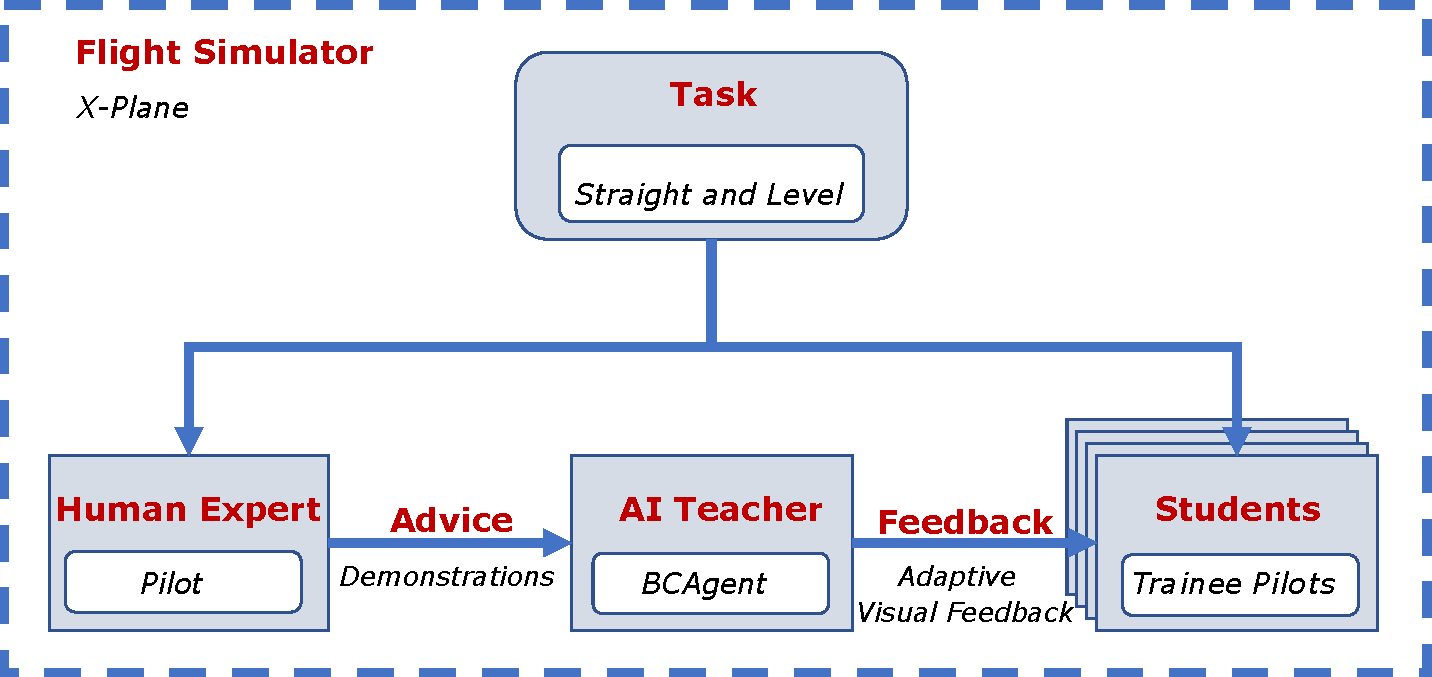
\includegraphics[width=\textwidth]{img/system1.pdf} 
		\caption{System Architecture} 
		\label{fig:system}
	\end{minipage}
\end{figure}
 
Our proposed intelligent tutoring system is shown in Figure~\ref{fig:system}. It includes four general components: (1) Task, (2) Human expert, (3) AI teacher, and (4) Students. The task is sampled from a curriculum of flying maneuvers useful for learning to fly. Both the pilot and students perform tasks using the flight simulator X-Plane.\footnote{https://developer.x-plane.com/article/airport-data-apt-dat-file-format-specification/} We use the fundamental flight maneuver ``straight and level"\footnote{\label{note1}Straight and level flight is a flight in which a constant heading and altitude are maintained. It is an essential flight maneuver used to form correct habits. All other flight maneuvers derive from straight and level.} as the target task. There is a human expert (pilot) who is adept in the task and can provide advice to train the AI teacher. After the AI teacher is trained to mimic the human teacher, the AI teacher is used to guide students by providing different types of feedback based on their performance on the target task. 
%Talk about this being a general framework?

\subsection{Modeling the Pilot: Agent Training}

We trained a decision-making agent to learn from pilot demonstrated trajectories. Experts demonstrated the``straight and level task" inside the flight simulator for $12.5$ minutes. They operate under visual flight rules, i.e, clear weather to fly towards the target. The target direction is changed between every trial demonstrated by the pilot to account for diversity in trajectory collection. The final dataset consists of $25$ trials of $30$ seconds each with a randomized goal between $\pm 30$ degrees from the starting heading.

After collecting demonstrations, we trained a behavior cloning (BC) agent~\cite{pomerleau1988alvinn} to mimic the pilot's policy. It is the simplest imitation learning technique where supervised learning is used to mimic the actions of an expert. The BC loss is defined as 
\begin{equation}
   L(\theta)=\sum_{i=1}^{N}||\pi_{\theta}(s_i)-\pi_e(s_i)||^2
   \label{bc_loss}
\end{equation}
where $\pi_{\theta}(s_i)$ is the current policy, $\pi_e(s_i)$ is the expert policy, $\theta$ is the training model parameter, and $N$ refers to the number of state-action pairs in the training set. We used stable baselines~\cite{stable-baselines3} to train the agent from demonstrations. The agent predicts the pitch and roll of the aircraft yoke. We evaluate the agent by measuring the average heading error over $10$ evaluation trials with randomized heading as seen in Figure~\ref{fig:evaluate} and terminate when the error stops improving.


% Imitation Learning is used to model the human expert in our framework. Demonstrations are collected from the pilot for the "straight and level" task. \\
% State-space: *(should we specify the entire list of observed variables here?if so I can paste in a list of the variables)* \\
% Action-space: *pitch and roll of the aircraft yoke*\\
% Specific imitation learning model used: *BC algorithm with default configuration outlined here: https://imitation.readthedocs.io/en/latest/algorithms/bc.html, probably what is more interesting is to discuss how trajectories are generated?*\\

% In order to evaluate the simulated teacher, we  compare the performance of this teacher against pilot performance. {We need to decide the plots and discuss them here}
\subsection{Deploying the Teacher and Guiding Students}

We deploy an agent when it makes similar decisions to the expert in previously unseen trials. Mimicking an expert pilot's behavior is not enough to teach students. A teacher should be able to detect students' mistakes and provide feedback to correct them. Therefore, we: (1)~Recorded students' poorly performed flights. (2)~Asked the pilots to prepare annotated critiques on errors made. (3)~Identified two main types of errors. (4)~Used simple distance metrics to decide whether the agent agreed or not with the student's decisions.
%\MET{System Architecture lists used 1) 2) but here we use (1) (2)... ?}

The identified student errors are due to (1) Not keeping altitude and airspeed constant and (2) Overshooting the target. To identify them, we compared how the agent and the student controlled the pitch and roll.  

Let $p_a(t), r_a(t), p_s(t),$ and~$r_s(t)$ represent the pitch and roll produced by the agent and the student at a given time~$t$. Then, for the first type of error:
\begin{equation}
  |p_a(t) - p_s(t)| \ge D_1  
  \label{eq_error1}
\end{equation}
where $D_1 \ge 0$ is a user-defined threshold. That is, the pitch difference is larger than the user-defined threshold. 

For the second type of error:
\begin{equation}
    |r_a(t) - r_s(t)| \ge D_2
    \label{eq_error2}
\end{equation}
where $D_2 \ge 0$ is a user-defined threshold. That is, the roll difference is larger than the user-defined threshold.

The agent uses Eqs.~\ref{eq_error1} and~\ref{eq_error2} to determine when to provide feedback. With respect to the type of feedback, this paper presents an instance of \emph{informative tutoring}, a type of formative feedback that presents verification feedback, error flagging, and strategic hints on how to proceed~\citep{shute:08}.
\begin{figure}[t]
	\begin{minipage}{1\linewidth}
		\centering \small
		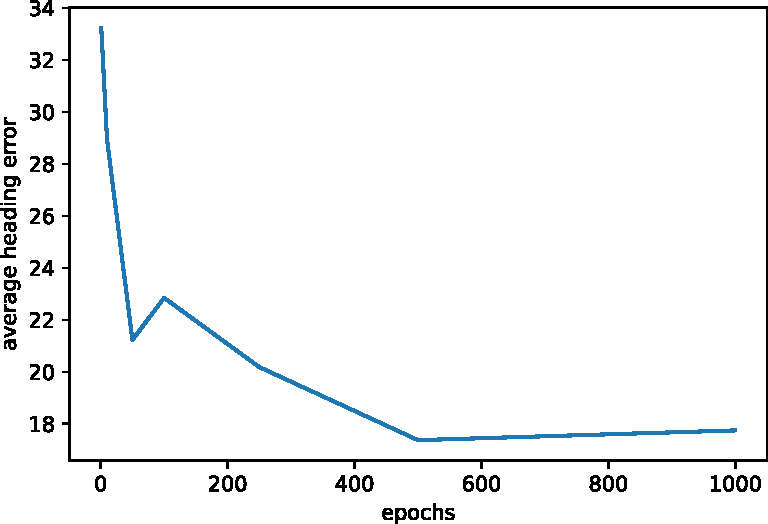
\includegraphics[width=\textwidth]{img/evaluation.pdf} 
		\caption{Average training time error of the behavior cloning teacher}
		\label{fig:evaluate}
	\end{minipage}
\end{figure}
\begin{figure}[t]
	\begin{minipage}{1\linewidth}
		\centering \small
		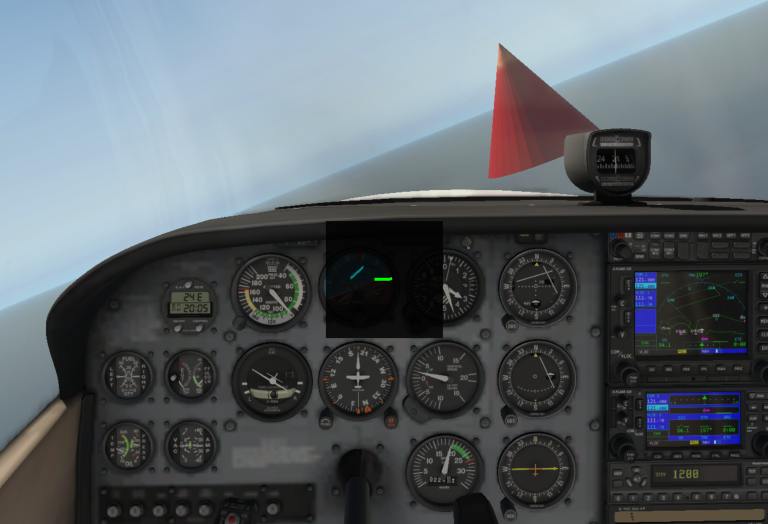
\includegraphics[width=\textwidth]{img/feedback.pdf} 
		\caption{Green and blue bars show visual tutor feedback}
		\label{fig:feedback}
	\end{minipage}
\end{figure}
Every time the user exceeds a threshold, the system displays a black square containing two lines denoting the user and the agent's status (Figure~\ref{fig:feedback}). The position $(x,y)$ of the middle of each line corresponds to $(r_a(t), p_a(t))$ and $(r_s(t), p_s(t))$ respectively, and the slope represents the roll angle.

This visualization shows how far apart the correct trajectory and position are. Instinctively, the student would aim to overlap both lines. Confirming the effectiveness of this and other types of feedback is part of future work.
 
\section{Conclusion and Future Work}
We presented an intelligent tutoring framework to autonomously train pilots inside a flight simulator using a simulated teacher. The teacher can provide different kinds of visual feedback to help students correct their mistakes. As future work, we will extend the simulated teacher to learn other complicated flight maneuvers like climbing and turning. We also plan to replace the BC teacher with reinforcement learning so that it can discover new policies not directly mentioned by the pilots. Lastly, we will study the impact of various kinds of feedback on student learning.

\bibliography{aaai23.bib}
\end{document}
